\chapter{Formatierungshilfen}
\label{KapitelFormatierungshilfen}
\index{Formatierungshilfen}
\index{Layout}

Dieses Kapitel beschreibt Formatierungshilfen und verschiedene Möglichkeiten, um das Layout von Dokumenten zu beeinflussen. 
Konkret stellt dieses Kapitel Befehle vor, um Absätze 
auszurichten, Zeilen umzubrechen,  
Abstände zwischen Wörtern und Zeichen einzufügen, sowie  
Leerräume aller Art zu erzeugen.

\section{Abstände von Wörtern und Zeichen}
\label{AbschnittWortabstandZeichenabstand}
\index{Wortabstand}
\index{Zeichenabstand}
\index{Zeichen!Abstand}

Der \LaTeX-Compiler ermöglicht es auf mehrere Arten Abstände zwischen Wörtern und
Zeichen zu realisieren. Die Möglichkeiten reichen von gewöhnlichen Leerzeichen und Abständen nach Satzzeichen bis zu Leerräumen aller Art.

\subsection{Abstände in Sätzen}
\label{AbschnittAbstaendeSaetzen}

\LaTeX\ interpretiert einen Punkt, genau wie ein Ausrufezeichen, ein Fragezeichen oder einen Doppelpunkt,
der nach einem Kleinbuchstaben oder einer Ziffer kommt, als das Ende eines Satzes.
Nach dem Punkt fügt \LaTeX\ automatisch einen Zwischenraum ein damit der neue Satz nicht direkt nach dem Punkt folgt. 

Kommt innerhalb eines Satzes ein Punkt vor, ist der vergleichsweise große Zwischenraum, der am Ende eines Satzes eingefügt wird, meist unerwünscht. Beispiele hierfür sind: \frqq Dr. Meier\flqq, \frqq i. Allg.\flqq\ oder \frqq u. a.\flqq.

In einem solchen Fall kann mit einer 
Tilde (\texttt{\textasciitilde})\index[cmd]{\texttt{\textbackslash textasciitilde}}  oder mit dem 
Befehl \verb!\!\texttt{\textvisiblespace}\index[cmd]{\texttt{\textbackslash textvisiblespace}}  
ein Wortabstand eingefügt werden, der kleiner ist als der übliche Abstand zwischen 
Sätzen. \verb!\!\texttt{\textvisiblespace} steht an dieser Stelle für einen Backslash, direkt gefolgt von einem Leerzeichen.


\fbox{\texttt{\textasciitilde}}

\fbox{\texttt{\textbackslash \textvisiblespace}}

Der Abstand, den \texttt{\textasciitilde} und
\verb!\!\texttt{\textvisiblespace} realisieren, ist identisch. Der einzige Unterschied zwischen beiden Vorgehensweisen ist, dass bei der Verwendung 
von \texttt{\textasciitilde} 
an der Stelle, an der dieses Zeichen eingesetzt wird, ein Zeilenumbruch\index{Zeilenumbruch}
vermieden wird, was besonders bei Namen sinnvoll ist.

\index{Abkürzungen}
Bei Abkürzungen empfiehlt sich 
der Einsatz eines Backslash und eines Kommas \verb!\,! um 
einen kleinen Zwischenraum einzufügen, bei dem ebenfalls kein Zeilenumbruch möglich ist.

Tabelle~\ref{Tabelle_Beispiele_Abstaende_Saetze} enthält einige Beispiele, bei denen ein Abstand, wie er zwischen Sätzen vorkommt, zu groß wäre.

\begin{table}[h!tb]
\centering
\caption{Beispiele für Abstände in Sätzen}
\label{Tabelle_Beispiele_Abstaende_Saetze}       % Give a unique label
\begin{tabular}{ll}
\hline
Beispiel & Quelltext \\
\hline
Prof.~Dr.~Meier & \texttt{Prof.\textasciitilde Dr.\textasciitilde Meier} \\
i.\,Allg. & \texttt{i.\textbackslash ,Allg.} \\
u.\,a. & \texttt{u.\textbackslash ,a.} \\
1.~Stock & \texttt{1.\textasciitilde Stock} \\
25~m & \texttt{25\textasciitilde m}\\ 
z.\,B. & \texttt{z.\textbackslash ,B.}\\
Dt.\,Bundesbahn & \texttt{Dt.\textbackslash ,Bundesbahn} \\
Dipl.\,Inf.\,(FH) & \texttt{Dipl.\textbackslash ,Inf.\textbackslash ,(FH)}\\
\hline
\end{tabular}
\end{table}


\subsection{Horizontale Abstände}
\label{Abschnitt:hspace}
\index{Abstand!horizontal}

Das manuelle Einfügen fester Abstände kann helfen, rasch ein Problem mit dem Layout zu lösen. Dennoch sollten Autoren dieses nur in Ausnahmefällen tun, weil es dem Prinzip der Trennung von Layout und Inhalt widerspricht. Zudem besteht die Gefahr, dass sich beim weiteren Einfügen von Texten, Bildern oder Tabellen im Dokument diese festen Abstände verschieben und dadurch den optischen Eindruck negativ beeinflussen.

Ein horizontaler Abstand kann unter anderem mit dem Befehl
\verb!\hspace!\index[cmd]{\texttt{\textbackslash hspace}} 
eingefügt werden.


\fbox{\texttt{\textbackslash hspace\{}\textsl{Abstand}\texttt{\}} }

Der Befehl erfordert die Angabe des 
einzufügenden Abstands inklusive einer Maßeinheit 
(siehe Abschnitt~\ref{sec:Massangaben}) in geschweiften Klammern.

Bei einem Zeilenumbruch oder 
ganz am Anfang einer Zeile wird 
\verb!\hspace! vom \LaTeX-Compiler ignoriert.

Eine Variante des Befehls \verb!\hspace! ist der Befehl 
\verb!\hspace*!. Dieser fügt im
Gegensatz zu \verb!\hspace! den Zwischenraum 
auch dann ein, wenn an der Stelle des
Befehlsaufrufs gerade ein Zeilenumbruch 
stattfindet oder wenn er am Anfang
einer Zeile aufgerufen wird. Einfach ausgedrückt: 
Die $\ast$-Form von 
\verb!\hspace! erzwingt den gewünschten, 
horizontalen Zwischenraum auf alle
Fälle. 

\fbox{\texttt{\textbackslash hspace*\{}\textsl{Abstand}\texttt{\}} }

Da jeweils ein Leerzeichen vor und
nach den Befehlen \verb!\hspace! und \verb!\hspace*! von \LaTeX\ mitgezählt wird, ist es für das Ergebnis nicht unerheblich, ob diese Befehle direkt nach einem Wort aufgerufen werden, oder ob sich noch ein Leerzeichen zwischen dem Wort 
und dem Befehl befindet.


% \texttt{1cm\textbackslash hspace\{1cm\}einfügen} \hfill 1cm\hspace{1cm}einfügen \\
% \texttt{1cm \textbackslash hspace\{1cm\}einfügen} \hfill 1cm \hspace{1cm}einfügen \\
% \texttt{1cm \textbackslash hspace\{1cm\} einfügen} \hfill 1cm \hspace{1cm} einfügen



% \begin{figure}[H]
\begin{minipage}[c]{0.6\textwidth}
\setlength{\parskip}{1em}
\frenchspacing
\begin{Verbatim}[frame=single]
1cm\hspace{1cm}einfügen \newline
1cm \hspace{1cm}einfügen \newline
1cm \hspace{1cm} einfügen
\end{Verbatim}
\end{minipage}
\hfill
\begin{minipage}[c]{0.36\textwidth}
\setlength{\parskip}{1em}
\frenchspacing
1cm\hspace{1cm}einfügen \\
1cm \hspace{1cm}einfügen \\
1cm \hspace{1cm} einfügen
\end{minipage}
% \end{figure}



Es ist auch möglich, den Befehlen \verb!\hspace! 
und \verb!\hspace*! negative Werte zu
übergeben. Dann wird \LaTeX\ die aktuelle
Position um die angegebene Länge zurücksetzen. In so einem Fall ist es allerdings
möglich, dass Text oder andere Inhalte überschrieben werden.



% \begin{figure}[H]
\begin{minipage}[c]{0.6\textwidth}
\setlength{\parskip}{1em}
\frenchspacing
\begin{Verbatim}[frame=single]
Einen Text\hspace{-1cm} überschreiben
\end{Verbatim}
\end{minipage}
\hfill
\begin{minipage}[c]{0.36\textwidth}
\setlength{\parskip}{1em}
\frenchspacing
Einen Text\hspace{-1cm} überschreiben
\end{minipage}
% \end{figure}

Weitere Befehle, die horizontale Abstände einfügen, sind \verb!\enskip!, \verb!\quad! und \verb!\qquad!. 

Wie groß der konkrete Abstand ist, der von diesen Befehlen eingefügt wird, hängt von der Länge der relativen Maßeinheit \verb!em! (siehe Abschnitt~\ref{sec:Massangaben}), also von der aktuell verwendeten Schriftart ab. 

Der Befehl \verb!\enskip! fügt einen horizontalen Abstand von einem halben \verb!em! ein, während die Befehle \verb!\quad! und \verb!\qquad! Abstände von einem bzw. zwei \verb!em! einfügen.

\begin{boxedminipage}{\textwidth}
\texttt{\textbackslash enskip} \\
\texttt{\textbackslash quad}  \\
\texttt{\textbackslash qquad} 
\end{boxedminipage}

Zudem gibt es noch die bereits in den Abschnitten~\ref{AbschnittAbstaendeSaetzen} und \ref{AbschnittZeilenAuffuellen} gezeigten Möglichkeiten zum Einfügen kleiner Wort- bzw. Zeichenabstände mit \verb!~!, \verb!\,!, \texttt{\textbackslash \textvisiblespace} und \verb!\hfill!.

\subsection{Vertikale Abstände}

\index{Abstand!vertikal}

Ein vertikaler Abstand kann unter anderem mit dem Befehl
\verb!\vspace!\index[cmd]{\texttt{\textbackslash vspace}} 
eingefügt werden. Der Befehl erfordert die Angabe des 
einzufügenden Abstands inklusive einer Maßeinheit 
(siehe Abschnitt~\ref{sec:Massangaben}) in geschweiften Klammern.


\fbox{\texttt{\textbackslash vspace\{}\textsl{Abstand}\texttt{\}} }



Eine Variante des Befehls \verb!\vspace! ist der Befehl 
\verb!\vspace*!. Dieser fügt im
Gegensatz zu \verb!\vspace! den Zwischenraum 
auch ein, wenn an der Stelle des
Befehlsaufrufs gerade ein Seitenumbruch 
stattfindet. Einfach ausgedrückt: 
Die $\ast$-Form von 
\verb!\vspace! erzwingt den gewünschten, 
vertikalen Zwischenraum auf alle
Fälle. 

\fbox{\texttt{\textbackslash vspace*\{}\textsl{Abstand}\texttt{\}} }

Beim Aufruf von \verb!\vspace! oder \verb!\vspace*! 
innerhalb eines Absatzes wird der \LaTeX-Compiler die aktuelle Zeile fertig 
mit Text befüllen und erst danach den 
vertikalen Zwischenraum einfügen.

Es ist auch möglich, einen negativen
Abstand einzufügen, und somit einen Bereich im Dokument \textsl{nach oben zu rücken}. 
Allerdings besteht auch hier -- genau wie bei \verb!\hspace*! -- das Risiko, Inhalte zu überschreiben.


Weitere Befehle zum einfügen vertikaler Abstände, auf die aus Platzgründen an dieser Stelle nicht weiter eingegangen wird, sind \verb!\smallskip!, \verb!\medskip! und \verb!\bigskip!, sowie \verb!\smallbreak!, \verb!\medbreak! und \verb!\bigbreak!. Bei diesen hängt der konkrete Abstand von der verwendeten Dokumentklasse (siehe Abschnitt~\ref{AbschnittDokumentklassen}) ab.


\subsection{Leerzeichen in Verbindung mit Satzzeichen -- Frenchspacing}
\index{Frenchspacing}


Einige Textverarbeitungsprogramme fügen nach einem Satzzeichen einen freien Zwischenraum ein, der größer ist als der normale Wortabstand. Diesen zusätzlichen Zwischenraum fügt auch \LaTeX\ ein, wenn es dazu mit dem Befehl \verb!\nonfrenchspacing! angewiesen wird. 


\fbox{\texttt{\textbackslash nonfrenchspacing}}
\index[cmd]{\texttt{\textbackslash nonfrenchspacing}}  

Die Wirksamkeit des Befehls erstreckt sich von seinem Aufruf (der an jeder beliebigen Stelle eines Dokuments sein kann) 
bis zum Ende des Dokuments oder bis zu einem 
Aufruf des Befehls \verb!\frenchspacing!. Dieser Befehl sorgt 
dafür, dass alle Wortabstände innerhalb einer Zeile gleich sind. 

\fbox{\texttt{\textbackslash frenchspacing}}
\index[cmd]{\texttt{\textbackslash doublebox}}  

Einen Vergleich der Auswirkungen der beiden Befehle zeigt Abbildung~\ref{Abbildungen_frenchspacing_nonfrenchspacing}.
Das Erweiterungspaket \verb!(n)german.sty! verwendet standardmäßig \verb!\frenchspacing!.

\begin{figure}[H]
\begin{minipage}[t]{0.48\textwidth}
\setlength{\parskip}{1em}
Mit \verb!\nonfrenchspacing!

\nonfrenchspacing 
Lorem ipsum dolor sit amet, consectetur adipiscing elit. Curabitur ullamcorper lacus ante, vitae bibendum odio sodales ac. Vestibulum quis pellentesque diam. Aliquam erat volutpat. Nunc gravida vestibulum lacus eu feugiat. Phasellus sit amet tellus nibh. Phasellus lobortis quam vel enim efficitur vestibulum. Duis eleifend eros a erat vehicula porta. Nam.
\end{minipage}
\hfill
\begin{minipage}[t]{0.48\textwidth}
\setlength{\parskip}{1em}
Mit \verb!\frenchspacing!

\frenchspacing
Lorem ipsum dolor sit amet, consectetur adipiscing elit. Curabitur ullamcorper lacus ante, vitae bibendum odio sodales ac. Vestibulum quis pellentesque diam. Aliquam erat volutpat. Nunc gravida vestibulum lacus eu feugiat. Phasellus sit amet tellus nibh. Phasellus lobortis quam vel enim efficitur vestibulum. Duis eleifend eros a erat vehicula porta. Nam.
\end{minipage}
\caption{Auswirkungen von \texttt{\textbackslash nonfrenchspacing} und \texttt{\textbackslash frenchspacing}}
\label{Abbildungen_frenchspacing_nonfrenchspacing}
\end{figure}


\subsection{Leerzeichen darstellen}
\index{Leerzeichen}

Die Eingabe eines Leerzeichens mit geschieht einfach durch die 
direkte Eingabe mit der Leertaste. 
Stehen im Quelltext mehrere Leerzeichen hintereinander, wird der
\LaTeX-Compiler dieses ignorieren und nur ein einziges Leerzeichen ausgeben.


Ein Leerzeichen kann auch mit Hilfe des Befehls 
\verb!\textvisiblespace! 
gesetzt werden. Der Befehl setzt folgendes Zeichen:
\glqq\textvisiblespace\grqq. So etwas ist z.~B. bei 
Dokumentationen hilfreich.

\fbox{\texttt{\textbackslash textvisiblespace}}
\index[cmd]{\texttt{\textbackslash textvisiblespace}}  

Eine alternative Möglichkeit, um ein Leerzeichen zu setzen, ist der 
Befehl \verb!\space!. Der erzeugt auch ein richtiges Leerzeichen, so wie dieses hier: \glqq\space\grqq

\fbox{\texttt{\textbackslash space}}
\index[cmd]{\texttt{\textbackslash space}}  

\subsection{Zeilen mit Zwischenräumen auffüllen}
\label{AbschnittZeilenAuffuellen}
\index{Zwischenraum}

Der Befehl \verb!\hfill! erzeugt einen Zwischenraum, der an der Stelle des Aufrufs so
viel freie Fläche erzeugt, dass die Zeile links und rechts bündig
abschließt. Der Befehl ist
eine Abkürzung für \verb!\hspace{\fill}! (siehe Abschnitt~\ref{Abschnitt:hspace}).

\fbox{\texttt{\textbackslash hfill}}
\index[cmd]{\texttt{\textbackslash hfill}}  

Diese Zeile:

\begin{Verbatim}[frame=single]
Anfang\hfill Ende
\end{Verbatim}

hat den folgenden Effekt:

Anfang\hfill Ende

Wird innerhalb einer Zeile mehrmals \verb!\hfill! aufgerufen, dann wird der
einzufügende Zwischenraum entsprechend geteilt, so dass jedes \verb!\hfill! ein
gleich großes Stück erhält. 

Diese Zeile:

\begin{Verbatim}[frame=single]
Anfang\hfill Mitte\hfill Ende
\end{Verbatim}

hat den folgenden Effekt:

Anfang\hfill Mitte\hfill Ende

Es ist auch möglich, mehrere \verb!\hfill! zu einem Zwischenraum zu
kombinieren. Jedes \verb!\hfill! einer Zeile bekommt seinen Anteil am möglichen Zwischenraum.

Diese Zeile:

\begin{Verbatim}[frame=single]
Eins\hfill Zwei\hfill\hfill Drei\hfill\hfill\hfill Ende
\end{Verbatim}

hat den folgenden Effekt:

Eins\hfill Zwei\hfill\hfill Drei\hfill\hfill\hfill Ende


\subsection{Zwischenräume mit Zeichen auffüllen}
\index{Zwischenraum}

Während \verb!\hfill! leere Zwischenräume erzeugt, füllen die Befehle \verb!\hrulefill! und \verb!\dotfill! Zwischenräume mit einer durchgezogenen bzw. mit einer gepunkteten Linie.

Ein Aufruf des
Befehls \verb!\hrulefill! 
füllt den gesamten Raum von der
Stelle, an der der Befehl aufgerufen wurde, 
bis zum Ende der aktuellen Zeile 
mit einem tiefen Strich. Das sieht so aus:\hrulefill

\fbox{\texttt{\textbackslash hrulefill}}
\index[cmd]{\texttt{\textbackslash hrulefill}}  

Die Arbeitsweise des Befehls \verb!\dotfill!
ist identisch zu \verb!\hrulefill!, allerdings füllt
\verb!\dotfill! den Raum bis zum Ende der aktuellen Zeile 
mit einer gepunkteten Linie. Das sieht so aus:\dotfill

\fbox{\texttt{\textbackslash dotfill}}
\index[cmd]{\texttt{\textbackslash dotfill}}  

Mit diesen einfachen Möglichkeiten, 
durchgezogene und gepunktete Linien zu 
erzeugen und Abstände zu beeinflussen, 
ist es zum Beispiel möglich, Formulare zum
Ausfüllen oder Umfragebögen zu erstellen. 
Der Quelltext von Listing~\ref{formularbeispiel} zeigt exemplarisch einen Ausschnitt aus einem Formular
mit typischen Feldern. Das Ergebnis des
Beispiels zeigt Abbildung~\ref{fig_formularbeispiel}.

\lstinputlisting[caption={Eine sinnvolles Beispiel zu \texttt{\textbackslash dotfill} und \texttt{\textbackslash hrulefill}},label=formularbeispiel, style=customlatex]{Beispiele/Formular/formular_beispiel.tex}

\begin{figure}[H]
	%     \centering
	% Abschneiden mit trim = liks unten rechts oben
	\fbox{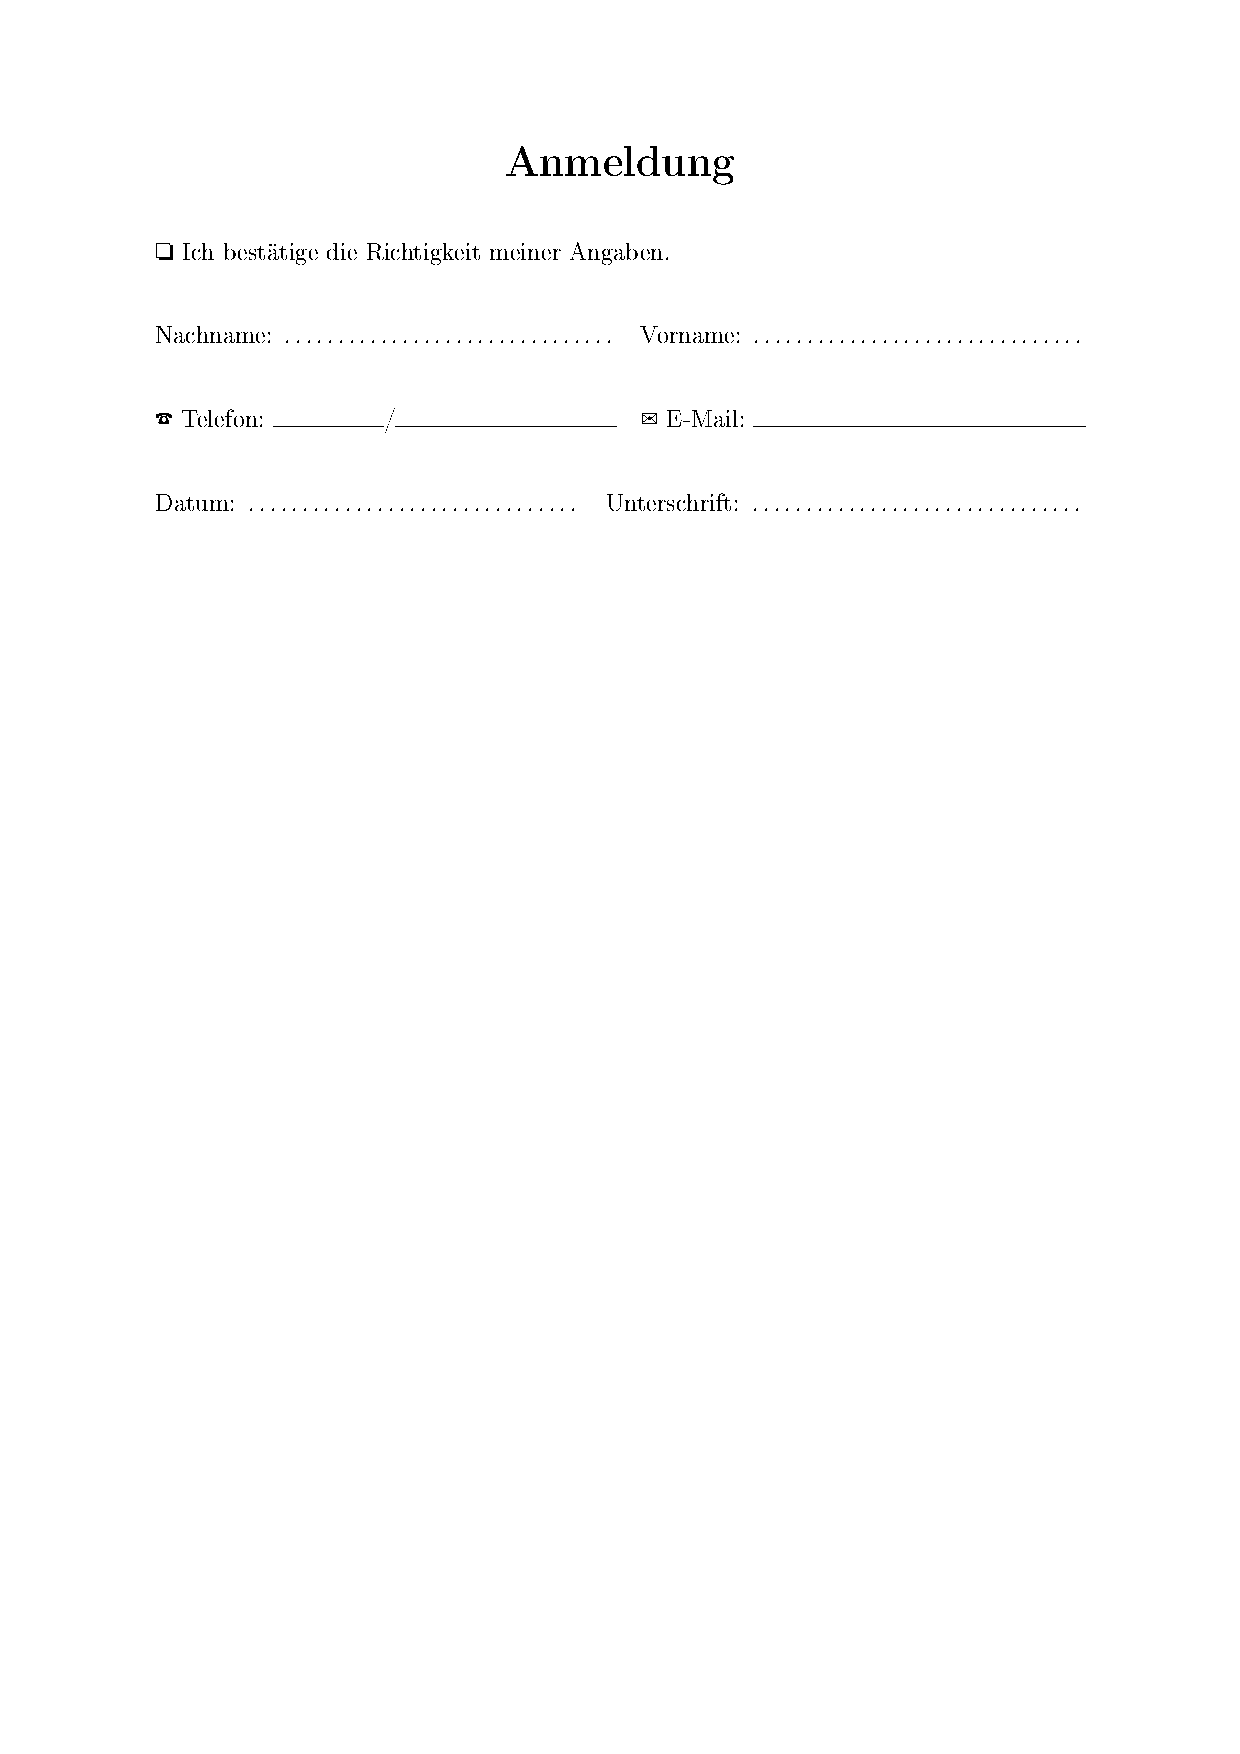
\includegraphics[page=1, clip, trim=2cm 20cm 2cm 2cm, width=.98\textwidth]{Beispiele/Formular/formular_beispiel.pdf}}
	\caption{Resultat von Listing~\ref{formularbeispiel}}
	\label{fig_formularbeispiel}
\end{figure}



\subsection{Grenzen des Textfeldes einhalten}
\index{Textfeld}

Je nach dem Layout des Dokuments und dem zu setzenden Text kann es passieren, das der \LaTeX-Compiler einzelne Wörter über das Textfeld herausragen lässt oder Wortabstände sehr groß erscheinen. In diesem Zusammenhang sind auch Warnungen des \LaTeX-Compilers wie \verb!Overfull \hbox...! und \verb!Underfull \hbox! zu verstehen.

Diese Warnungen können auch im Zusammenhang mit übergroßen oder zu geringen Abständen zwischen Absätzen aufkommen. In diesem Fall enthält die Warnung nicht ein \verb!\hbox!, sondern ein \verb!\vbox!.

Ein Überschreiten des Textfeldes verhindert ein Befehl \verb!\sloppy! in der Präambel des Dokuments. 

\fbox{\texttt{\textbackslash sloppy}}
\index[cmd]{\texttt{\textbackslash sloppy}}  

Dieser Befehl sorgt dafür, das \LaTeX\ bereit ist, Wortabstände wenn nötig weiter zu dehnen als das üblich der Fall ist.

Dem Autor dieser Zeilen ist bewusst, das der Befehl \verb!\sloppy! nicht nur Fans hat, sondern auch an einigen Stellen von seiner
Verwendung abgeraten wird~\cite{LaTeXSuendenregisterLink}. Diese Ablehnung teilt der Autor dieses Werkes aber explizit nicht.

\subsection{Trennungsregeln}
\index{Trennungsregel}

Bei Verwendung der Erweiterungspakete \verb!german! oder \verb|ngerman| hält sich der \LaTeX-Compiler an die deutschen Trennungsregeln.
Gerade bei Fremdwörtern kann es jedoch vorkommen, das Autoren aktiv in die Worttrennung eingreifen müssen.

Eine Möglichkeit ist es, in betreffenden Wörtern mit Hilfe von \verb|\-| manuell Trennungshilfen dort zu definieren, wo Sie ein Wort getrennt
sehen möchten. In der Praxis kann so etwas 
wie folgt aussehen:

\verb!... kommt es zu Durch\-schnitts\-verschiebungen ...!

Diese Trennungshilfen werden nur dann an der konkreten Stelle vom \LaTeX-Compiler berücksichtigt, wenn das Wort am 
Ende einer Zeile steht und getrennt werden muss. Ansonsten sind im fertigen Dokument die im Quelltext eingefügten Trennungshilfen 
zu keiner Zeit erkennbar.

Kommen ein oder mehrere Wörter mit aus Sicht des \LaTeX-Compilers unklarer Worttrennung\index{Worttrennung} mehrfach in einem Dokument vor, ist es sinnvoll
in der Präambel des Dokuments mit dem Befehl \verb!\hyphenation! Trennungsregeln für diese Wörter für das gesamte Dokument zu definieren. 

\fbox{\texttt{\textbackslash hyphenation\{}\textsl{Wort\_1} \textsl{Wort\_2} ... \textsl{Wort\_n}\texttt{\}}}

Die Wörter sind durch Leerzeichen voneinander abgegrenzt. 
Um die Lesbarkeit des Quelltextes an dieser Stelle zu verbessern, kann auch jedes Wort mit einer neuen Zeile beginnen.
In den Wörtern sind die Stellen, an denen Sie dem \LaTeX-Compiler Worttrennungen erlauben, mit Bindestrichen markiert.
Ein Beispiel könnte wie folgt aussehen:

\begin{Verbatim}[frame=single]
\hyphenation{
DHCP-Dis-cover
Durch-schnitts-ver-schiebung 
Pegel-wechsel 
Signal-pegel 
Maxi-mum
Topo-lo-gie
}
\end{Verbatim}


\section{Absätze zentrieren, nach einer Seite ausrichten oder einrücken}

Standardmäßig setzt der \LaTeX-Compiler Texte im \textsl{Blocksatz}\index{Blocksatz}. 
Diese Layoutform ist die am besten lesbare und optisch ansprechendste.
Zudem existiert die Möglichkeit, Text linksbündig, rechtsbündig, zentriert oder beidseitig eingerückt zu setzen. 
Text, der nur nach einer Seite bündig ist, heißt auch \textsl{Flattersatz}\index{Flattersatz}.

Linksbündiger Text ist
ähnlich gut lesbar wie Blocksatz, aber optisch weniger ansprechend. 
Rechtsbündige Texte sind in einigen Kulturkreisen der Standard, im deutschen Sprachraum aber nur selten anzutreffen.
Das zentrieren (also mittiges setzen) von Text ist ein 
häufig angewandtes Stilmittel, um etwas hervorzuheben (z.~B. eine Überschrift).

Zur Realisierung von zentriertem, linksbündigem,
rechtsbündigem oder beidseitig eingerücktem Text existieren jeweils Umgebungen und Befehle.

\subsection{Zentrierter Text}
\index{Zentrierter Text}
\index{Text!zentriert}


% \begin{figure}[H]
\begin{minipage}[t]{0.48\textwidth}
\setlength{\parskip}{1em}
\frenchspacing
% \begin{center}
Mit der Umgebung \verb!center!\index[cmd]{\texttt{center}}  
werden beliebige Inhalte (Text, Abbildungen, Tabellen, etc.) zentriert gesetzt.
Alternativ existiert der Befehl \verb!\centering!\index[cmd]{\texttt{\textbackslash centering}}  , der den 
nachfolgenden
Text zentriert setzt. 

Der nebenstehende zentriert gesetzte Text wurde mit der Umgebung \verb!center! erzeugt.
% \end{center}
\end{minipage}
\hfill
\begin{minipage}[t]{0.48\textwidth}
\setlength{\parskip}{1em}
\frenchspacing
\begin{center}
Lorem ipsum dolor sit amet, consectetur adipiscing elit. Curabitur ullamcorper lacus ante, vitae bibendum odio sodales ac. Vestibulum quis pellentesque diam. Aliquam erat volutpat. Nunc gravida vestibulum lacus eu feugiat. Phasellus sit amet tellus nibh. Phasellus lobortis quam vel enim efficitur vestibulum. Duis eleifend eros a erat vehicula porta. Nam.
\end{center}
% \caption{Zentrierter Text}
% \label{Abbildungen_zentrierter_Text}
\end{minipage}
% \end{figure}



\begin{boxedminipage}{\textwidth}
\texttt{\textbackslash begin\{center\}}\dots\texttt{\textbackslash end\{center\}}\\
\texttt{\textbackslash centering} 
\end{boxedminipage}



\subsection{Linksbündiger Text}
\index{Linksbündiger Text}
\index{Text!linksbündig}

% \begin{figure}[H]
\begin{minipage}[t]{0.48\textwidth}
\setlength{\parskip}{1em}
\frenchspacing
% \begin{center}
Inhalte linksbündig im Flattersatz setzen die 
Umgebung \verb!flushleft! und alternativ der Befehl \verb!\raggedleft!.
\index[cmd]{\texttt{\textbackslash flushleft}}  
\index[cmd]{\texttt{\textbackslash raggedleft}}  

Der nebenstehende linksbündig gesetzte Text wurde mit der Umgebung \verb!flushleft! erzeugt.
% \end{center}
\end{minipage}
\hfill
\begin{minipage}[t]{0.48\textwidth}
\setlength{\parskip}{1em}
\frenchspacing
\begin{flushleft}
Lorem ipsum dolor sit amet, consectetur adipiscing elit. Curabitur ullamcorper lacus ante, vitae bibendum odio sodales ac. Vestibulum quis pellentesque diam. Aliquam erat volutpat. Nunc gravida vestibulum lacus eu feugiat. Phasellus sit amet tellus nibh. Phasellus lobortis quam vel enim efficitur vestibulum. Duis eleifend eros a erat vehicula porta. Nam.
\end{flushleft}
\end{minipage}
% \end{figure}




\begin{boxedminipage}{\textwidth}
\texttt{\textbackslash begin\{flushleft\}}\dots\texttt{\textbackslash end\{flushleft\}}\\
\texttt{\textbackslash raggedleft} 
\end{boxedminipage}


\subsection{Rechtsbündiger Text}
\index{Rechtsbündiger Text}
\index{Text!rechtsbündig}


% \begin{figure}[H]
\begin{minipage}[t]{0.48\textwidth}
\setlength{\parskip}{1em}
\frenchspacing
% \begin{center}
Inhalte rechtsbündig im Flattersatz setzen die 
Umgebung \verb!flushright! und alternativ der Befehl \verb!\raggedright!.
\index[cmd]{\texttt{\textbackslash flushright}}  
\index[cmd]{\texttt{\textbackslash raggedright}}  

Der nebenstehende rechtsbündig gesetzte Text wurde mit der Umgebung \verb!flushright! erzeugt.
% \end{center}
\end{minipage}
\hfill
\begin{minipage}[t]{0.48\textwidth}
\setlength{\parskip}{1em}
\frenchspacing
\begin{flushright}
Lorem ipsum dolor sit amet, consectetur adipiscing elit. Curabitur ullamcorper lacus ante, vitae bibendum odio sodales ac. Vestibulum quis pellentesque diam. Aliquam erat volutpat. Nunc gravida vestibulum lacus eu feugiat. Phasellus sit amet tellus nibh. Phasellus lobortis quam vel enim efficitur vestibulum. Duis eleifend eros a erat vehicula porta. Nam.
\end{flushright}
\end{minipage}
% \end{figure}




\begin{boxedminipage}{\textwidth}
\texttt{\textbackslash begin\{flushright\}}\dots\texttt{\textbackslash end\{flushright\}}\\
\texttt{\textbackslash raggedright} 
\end{boxedminipage}



\subsection{Beidseitig eingerückter Text}
\index{eingerückter Text}
\index{Text!eingerückt}

Besonders bei Zitaten ist es optisch ansprechend, wenn der Text beidseitig gleich weit eingerürückt ist, um ihn dadurch hervorzuheben. Zu diesem Zweck 
existierenden die beiden Umgebungen \verb!quote! und alternativ \verb!quotation!.
\index[cmd]{\texttt{quote}}  
\index[cmd]{\texttt{quotation}}  

Der folgende beidseitig gleich weit eingerückt gesetzte Text wurde mit der Umgebung \verb!quote! erzeugt.

\begin{quote}
	Lorem ipsum dolor sit amet, consectetur adipiscing elit. 
	
	Curabitur ullamcorper lacus ante, vitae bibendum odio sodales ac. 
	
	Vestibulum quis pellentesque diam. Aliquam erat volutpat. 
\end{quote}

Die Umgebung \verb!quote! fügt automatisch zwischen Absätzen einen vertikalen Abstand ein und rückt die erste Zeile eines jeden Absatzes nicht ein. 

\fbox{
	\texttt{\textbackslash begin\{quote\}}\dots\texttt{\textbackslash end\{quote\}}
}

Das Verhalten von \verb!quote! entspricht damit dem Standard im deutschen Sprachraum.

Der folgende beidseitig gleich weit eingerückt gesetzte Text wurde mit der Umgebung \verb!quotation! erzeugt.

\begin{quotation}
	Lorem ipsum dolor sit amet, consectetur adipiscing elit. 
	
	Curabitur ullamcorper lacus ante, vitae bibendum odio sodales ac. 
	
	Vestibulum quis pellentesque diam. Aliquam erat volutpat. 
\end{quotation}

Die Umgebung \verb!quotation! rückt die erste Zeile eines jeden Absatzes ein und verzichtet dafür auf den vertikalen Abstand zwischen Absätzen. 

\fbox{\texttt{\textbackslash begin\{quotation\}}\dots\texttt{\textbackslash end\{quotation\}}}

Das Verhalten von \verb!quotation! entspricht damit dem Standard im anglo-amerikanischen Sprachraum.




\section{Zeilenumbrüche}
\index{Zeilenumbruch} 

Ein Zeilenumbruch 
kann an beliebiger Stelle im Text mit dem
Befehl \verb!\\!\index[cmd]{\texttt{\textbackslash\textbackslash}} realisiert werden. Zudem ist es möglich, mit dem 
optionalen Parameter \textsl{Abstand} den vertikalen Zwischenraum zur nächsten Zeile anzugeben. Wenn durch
den Parameter \textsl{Abstand} ein Seitenumbruch zustande kommt, dann wird 
der Inhalt von \textsl{Abstand} vom \LaTeX-Compiler ignoriert und die nächste Seite 
beginnt mit der nächsten Textzeile. 

\begin{boxedminipage}{\textwidth}
	\texttt{\textbackslash \textbackslash[}\textsl{Abstand}\texttt{]}
\end{boxedminipage}


Eine Variante des Befehls \verb!\\! ist der Befehl 
\verb!\\*!. Dieser verhindert, dass nach
dem Zeilenumbruch ein Seitenwechsel 
vor der nächsten Textzeile erscheint.


\begin{boxedminipage}{\textwidth}
	\texttt{\textbackslash \textbackslash*[}\textsl{Abstand}\texttt{]} 
\end{boxedminipage}


Enthält ein Dokument beispielsweise den Befehl 
\verb!\\[1cm]!, dann wird der \LaTeX-Compiler einen Zeilenumbruch 
mit einen vertikalen Zeilenabstand von 1\,cm 
einfügen. Kommt durch diesen  Befehl ein 
Seitenumbruch zustande, dann 
wird der \LaTeX-Compiler auf der neuen Seite die 
dem Befehl vorangegangene Zeile 
setzen, dann den 1\,cm großen Abstand einfügen und danach die nächste Zeile. 


Eine weitere Variante ist der 
Befehl \verb!\newline!\index[cmd]{\texttt{\textbackslash newline}}, 
dessen Verhalten mit dem des Befehls \verb!\\! identisch ist. 
Mit \verb!\newline! ist es allerdings nicht möglich, den 
Zwischenraum zur nächsten Zeile zu definieren.


\fbox{\texttt{\textbackslash newline}}




\section{Seitenumbrüche}
\index{Seitenumbruch}

Genau wie beim Zeilenumbruch wird auch 
der Seitenumbruch vom \LaTeX-Compiler selbst
vorgenommen. Er versucht eventuell vorhandene
Gleitobjekte wie Bilder und Tabellen an der geeignetsten Position 
zu setzen, damit es nicht zu den so genannten
\textsl{Hurenkindern} oder \textsl{Schusterjungen} kommt (siehe Abschnitt~\ref{Absatzabstand}),

In seltenen Fällen kann es aber sinnvoll sein,
einen Seitenumbruch an einer bestimmten Stelle anzuweisen.


Der Befehl \verb!\newpage!\index[cmd]{\texttt{\textbackslash newpage}}  
beendet bei einem einspaltigen Seitenlayout 
die aktuelle Seite und bei einem zweispaltigen 
Layout die aktuelle Spalte. 


\fbox{\texttt{\textbackslash newpage}}

Das manuelle Umbrechen der aktuelle Seite bei eine zweispaltigen Seitenlayout (Klassenoption \verb!twocolumn! oder Befehl \verb!\twocolumn!) geschieht mit dem Befehl \verb!\clearpage!.\index[cmd]{\texttt{\textbackslash clearpage}}  

\fbox{\texttt{\textbackslash clearpage}}

Bei einem doppelseitigem Layout (Klassenoption \verb!twoside!) geschieht das manuelle Umbrechen der aktuelle Seite mit dem Befehl 
\verb!\cleardoublepage!.\index[cmd]{\texttt{\textbackslash cleardoublepage}}  
Dieser garantiert, das die nächste Seite, auf der sich Inhalte befinden, eine ungerade (linke) Seite ist.

\fbox{\texttt{\textbackslash cleardoublepage}}

In bestimmten Situationen kann es hilfreich sein, einen Seitenumbruch an einer bestimmten Stelle zu untersagen. Zu diesem Zweck existiert der Befehl \verb!nopagebreak!.

\fbox{\texttt{\textbackslash nopagebreak}}
\index[cmd]{\texttt{\textbackslash nopagebreak}}  
